\documentclass[authoryear, 12pt,5p, times]{elsarticle}
%\usepackage[hypcap]{caption}
%\geometry{margin=0.95in,top=1.4in,bottom=1.4in}
\geometry{margin=1in,top=1.3in,bottom=1.3in}
\usepackage{float}
\usepackage{amsmath}
\usepackage[hidelinks]{hyperref} 
 \usepackage{gensymb}
\usepackage{subcaption}
\usepackage{url}
%\renewcommand\thefootnote{\fnsymbol{\dagger}}
\usepackage[symbol*]{footmisc}
\newcommand{\rpm}{\raisebox{.2ex}{$\scriptstyle\pm$}}
\begin{document}
%\footnote{This is a footnote}
\begin{frontmatter}
\title{Asteroid Astrometry from CCD Images}
\author{\today \\ \quad \\Jung Lin (Doris) Lee\\ dorislee@berkeley.edu\\Group partners: Jennifer Ito, Manuel Silvia\\Prof. James Graham, UGSI Heechan Yuk, Isaac Domagalski}
	\begin{abstract}
astrometry for asteroid name..etc
	\end{abstract}
\end{frontmatter}
\section{Introduction}

\section{Data Reduction}
	
	\subsection{Bias Correction}
		\textbf{\paragraph{Overscan correction}}
		Overscan pixels are	32 pseudo-pixels generated by the data aquiscition software of the reader (?). Resulting in an array size of 1024
We take the median value of the 32 pseudo-pixels and subtract them from the actual data. This eliminates the constant offset from the every pixel reading. 
	
		\textbf{\paragraph{Bias subtraction}}
		The more bias subtraction the better since bias is Poisson, so falls off as $1/\sqrt{N}$
	\subsection{Flat Correction}
			We took 12 flat frames for the B,V,R,I filters on the observing session on October 16, 2014 at dusk time. The exposure time was adjusted for every frame to accommodate for the sky's changing brightness. Every pixel on the 1024-by-1024 image is processed by : 
			\begin{equation}
			\frac{\text{image}-\text{dark}}{\text{flat}}\times\text{median(flat)}
			\end{equation}
		 As shown in the equation, we first dark-subtract from the image so that the intensity is linearly proportional to the number of photon counts then we divide by the flat in order to scale for the pixel-by-pixel . Then, this is multiplied by a scalar value that is representative of the magnitude of the flat field data that we are subtracting off. The median value is chosen because unlike the mean its value is not skewed due to the outliers (i.e. bad pixel and columns).

	\begin{figure}[h!]
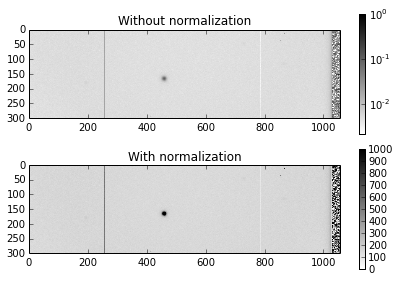
\includegraphics[width=0.5\textwidth]{figures/normalization}
\caption{Without normalization, the image requires a logarithmic stretch on the color bar scale to distinguish the asteroid and the background since it has to accommodate for the range of decimal values resulting from the division. With normalization, the image can be viewed on a linear scale with a lower intensity limit of 0 and upper limit of 1000.}
\label{normalization}
\end{figure}

	
\section{Astrometry}
	\subsection{Centroid Finding}
		\subsubsection{Algorithm}
	\subsection{General Least Square Method}

\section{Conclusion}

 \section{References}
%\bibliographystyle{elsarticle-harv}
\begin{itemize}
\item Howell, Steve,  \textit{Handbook of CCD Astronomy}, 2nd Edition. Cambridge University Press, 2006.
\item Wall, J. V. and Jenkins, C.R., \textit{Practical Statistics for Astronomers}, Cambridge University Press, 2002.
\item Press, William H., and William T. Vetterling. \textit{Numerical Recipes in C: The Art of Scientific Computing}. Cambridge University Press, 1992. 
\end{itemize}
\end{document}
